\documentclass[10pt]{beamer}

% Packages
\usepackage[utf8]{inputenc}
\usepackage[T1]{fontenc}
\usepackage{amsmath, amssymb, amsthm}
\usepackage{graphicx}
\usepackage{booktabs}
\usepackage{hyperref}
\usepackage{tikz}
\usetikzlibrary{shapes,arrows,positioning}

% Theme settings
\usetheme{default}
\usecolortheme{default}
\usefonttheme{professionalfonts}

\definecolor{ImperialBlue}{RGB}{0, 62, 116}
\definecolor{DarkGray}{RGB}{51, 51, 51}
\definecolor{LightGray}{RGB}{245, 245, 245}
\definecolor{AccentOrange}{RGB}{214, 96, 77}
\definecolor{AccentGreen}{RGB}{46, 139, 87}

% Apply colors
\setbeamercolor{frametitle}{fg=ImperialBlue, bg=white}
\setbeamercolor{title}{fg=ImperialBlue}
\setbeamercolor{structure}{fg=ImperialBlue}
\setbeamercolor{normal text}{fg=DarkGray}
\setbeamercolor{block title}{fg=white, bg=ImperialBlue}
\setbeamercolor{block body}{fg=DarkGray, bg=LightGray}
\setbeamercolor{itemize item}{fg=ImperialBlue}
\setbeamercolor{enumerate item}{fg=ImperialBlue}

% Remove navigation symbols
\setbeamertemplate{navigation symbols}{}

% Customize frame title
\setbeamertemplate{frametitle}{
  \vspace{0.5em}
  \insertframetitle
  \vspace{0.3em}
}

% Customize itemize
\setbeamertemplate{itemize items}[circle]
\setlength{\leftmargini}{1.5em}

% Footer
\setbeamertemplate{footline}{
  \leavevmode%
  \hbox{%
  \begin{beamercolorbox}[wd=.333333\paperwidth,ht=2.25ex,dp=1ex,left]{author in head/foot}%
    \hspace{1em}\usebeamerfont{author in head/foot}\insertshortauthor
  \end{beamercolorbox}%
  \begin{beamercolorbox}[wd=.333333\paperwidth,ht=2.25ex,dp=1ex,center]{title in head/foot}%
    \usebeamerfont{title in head/foot}\insertshorttitle
  \end{beamercolorbox}%
  \begin{beamercolorbox}[wd=.333333\paperwidth,ht=2.25ex,dp=1ex,right]{date in head/foot}%
    \usebeamerfont{date in head/foot}\insertshortdate{}\hspace*{2em}
    \insertframenumber{} / \inserttotalframenumber\hspace*{2ex} 
  \end{beamercolorbox}}%
  \vskip0pt%
}

% Commands for highlighting
\newcommand{\emphbox}[1]{\colorbox{LightGray}{\textcolor{DarkGray}{#1}}}
\newcommand{\highlight}[1]{\textcolor{AccentOrange}{\textbf{#1}}}
\newcommand{\good}[1]{\textcolor{AccentGreen}{#1}}
\newcommand{\bad}[1]{\textcolor{AccentOrange}{#1}}

%----------------------------------------------------------------------------------------
\title{Digital Ownership and Tokenization}
\subtitle{ECOM215: Blockchain Economics and Digital Assets}
\author{Dr Daniele Bianchi}
\institute{Queen Mary, University of London}
\date{Semester B, 2025/2026}
%----------------------------------------------------------------------------------------

\begin{document}

\AtBeginSection[]{
  \begin{frame}[plain]
    \vfill
    \begin{center}
      {\Large\color{ImperialBlue}\insertsection}
    \end{center}
    \vfill
  \end{frame}
}

\begin{frame}[plain]
  \titlepage
\end{frame}

\begin{frame}{Today's Agenda}
  \tableofcontents
\end{frame}

%----------------------------------------------------------------------------------------
\section{What is Tokenization?}
%----------------------------------------------------------------------------------------

\begin{frame}{The Big Picture}
  \textbf{Core idea}: Represent ownership of assets as tokens on a blockchain.
  
  \vspace{1em}
  \textbf{What can be tokenized?}
  \begin{itemize}
    \item Digital art and collectibles (NFTs)
    \item Financial securities (stocks, bonds)
    \item Real estate
    \item Commodities
    \item Credentials and identity
    \item Virtually any asset with defined ownership
  \end{itemize}
  
  \vspace{1em}
  \textbf{Why put ownership on-chain?}
  \begin{itemize}
    \item \textbf{Programmability}: Automate dividends, royalties, compliance
    \item \textbf{24/7 trading}: No market hours, instant settlement
    \item \textbf{Fractional ownership}: Own 0.01\% of a building
    \item \textbf{Transparency}: Verifiable ownership history
    \item \textbf{Global access}: Anyone with a wallet can participate
  \end{itemize}
\end{frame}

\begin{frame}{Fungible vs Non-Fungible Tokens}
  
  \begin{block}{Fungible}
    Each unit is identical and interchangeable. One unit can be swapped for any other unit of the same type.
  \end{block}
  
  \textbf{Examples}: Bitcoin, ETH, USDC, company shares
  
  \vspace{1em}
  \begin{block}{Non-Fungible}
    Each token is unique and not interchangeable. Tokens have distinct properties or identifiers.
  \end{block}
  
  \textbf{Examples}: Digital art, event tickets, property deeds, credentials
  
  \vspace{1em}
  \textbf{Key insight}: Fungibility is about \textit{substitutability}. Can you swap one for another without caring which specific one you have?
\end{frame}

\begin{frame}{What Does a Token Actually Contain?}
  A token on a blockchain typically contains:
  
  \vspace{0.5em}
  \textbf{On-chain} (stored directly on blockchain):
  \begin{itemize}
    \item Token ID (unique identifier)
    \item Owner address
    \item Contract address
    \item Transfer history
  \end{itemize}
  
  \vspace{0.5em}
  \textbf{Off-chain} (stored elsewhere, linked via URI):
  \begin{itemize}
    \item Image/media file
    \item Description and attributes
    \item Additional metadata
  \end{itemize}
  
  \vspace{1em}
  \highlight{Critical point}: Most NFTs don't store the actual image on-chain---too expensive. They store a \textit{link} to the image.
  
  \vspace{0.5em}
  \textbf{Risk}: If the server hosting the image goes down, you own... a broken link.
\end{frame}

\begin{frame}{Metadata Storage Options}
  
  \begin{center}
 \resizebox{1\textwidth}{!}{\begin{tabular}{lll}
    \toprule
    \textbf{Storage} & \textbf{Pros} & \textbf{Cons} \\
    \midrule
    On-chain & Permanent, decentralised & Very expensive, size limits \\
    IPFS & Decentralised, content-addressed & Needs pinning, can disappear \\
    Centralised server & Cheap, flexible & Single point of failure \\
    Arweave & Permanent, paid once & Cost, smaller ecosystem \\
    \bottomrule
  \end{tabular}}
  \end{center}
  
  \vspace{1em}
  \textbf{IPFS} (InterPlanetary File System): Decentralised storage where files are addressed by their content hash, not location.
  
  \vspace{0.5em}
  \textbf{Best practice}: Use IPFS or Arweave for important metadata. Many early NFT projects used centralised servers---some images are already lost.
\end{frame}

%----------------------------------------------------------------------------------------
\section{Token Standards}
%----------------------------------------------------------------------------------------

\begin{frame}{Why Standards Matter}
  Token standards define:
  \begin{itemize}
    \item How tokens are created (minted)
    \item How ownership is tracked
    \item How transfers work
    \item What functions wallets and marketplaces can expect
  \end{itemize}
  
  \vspace{1em}
  \textbf{Interoperability}: A standard means any wallet or marketplace can interact with any token following that standard.
  
  \vspace{1em}
  \textbf{Main Ethereum standards}:
  \begin{itemize}
    \item \textbf{ERC-20}: Fungible tokens (most cryptocurrencies)
    \item \textbf{ERC-721}: Non-fungible tokens (unique items)
    \item \textbf{ERC-1155}: Multi-token standard (both fungible and non-fungible)
  \end{itemize}
  
  \vspace{0.5em}
  Other chains have equivalent standards (e.g., SPL on Solana).
\end{frame}

\begin{frame}{ERC-20: Fungible Tokens}
  The standard for fungible tokens on Ethereum (2015).
  
  \vspace{0.5em}
  \textbf{Key functions}:
  \begin{itemize}
    \item \texttt{totalSupply()}: How many tokens exist?
    \item \texttt{balanceOf(address)}: How many does this address own?
    \item \texttt{transfer(to, amount)}: Send tokens to another address
    \item \texttt{approve(spender, amount)}: Allow another contract to spend your tokens
  \end{itemize}
  
  \vspace{1em}
  \textbf{Examples}: USDC, USDT, UNI, LINK, most DeFi tokens
  
  \vspace{1em}
  \textbf{Why it matters}: ERC-20 enabled the ICO boom, DeFi composability, and standardised how tokens work across the ecosystem.
\end{frame}

\begin{frame}{ERC-721: Non-Fungible Tokens}
  The standard for NFTs on Ethereum (2018).
  
  \vspace{0.5em}
  \textbf{Key differences from ERC-20}:
  \begin{itemize}
    \item Each token has a unique \texttt{tokenId}
    \item \texttt{ownerOf(tokenId)}: Who owns this specific token?
    \item \texttt{tokenURI(tokenId)}: Where is this token's metadata?
    \item Tokens are indivisible---you can't send 0.5 of an NFT
  \end{itemize}
  
  \vspace{1em}
  \textbf{Examples}: CryptoPunks, Bored Apes, most digital art NFTs
  
  \vspace{1em}
  \textbf{Limitation}: Each token type requires a separate transaction. Minting 10,000 NFTs = 10,000 transactions (expensive).
\end{frame}

\begin{frame}{ERC-1155: Multi-Token Standard}
  A more efficient standard that supports both fungible and non-fungible tokens in one contract (2019).
  
  \vspace{0.5em}
  \textbf{Key advantages}:
  \begin{itemize}
    \item Batch transfers: Send multiple token types in one transaction
    \item Mixed fungibility: Some IDs can be fungible, others unique
    \item Gas efficient: Significantly cheaper for games and collections
  \end{itemize}
  
  \vspace{1em}
  \textbf{Use case}: Gaming
  \begin{itemize}
    \item Token ID 1: Gold coins (fungible---1 million exist)
    \item Token ID 2: Health potions (fungible---10,000 exist)
    \item Token ID 3: Legendary sword (non-fungible---only 1 exists)
  \end{itemize}
  
  \vspace{0.5em}
  All managed in one contract, transferable in batches.
\end{frame}

\begin{frame}{Token Standards Comparison}
  \begin{center}
  \begin{tabular}{lccc}
    \toprule
    & \textbf{ERC-20} & \textbf{ERC-721} & \textbf{ERC-1155} \\
    \midrule
    Fungibility & Fungible & Non-fungible & Both \\
    Divisible & Yes & No & Configurable \\
    Batch transfer & No & No & Yes \\
    Gas efficiency & Medium & Low & High \\
    Use case & Currencies, shares & Art, collectibles & Gaming, mixed \\
    \bottomrule
  \end{tabular}
  \end{center}
  
  \vspace{1em}
  \textbf{Choosing a standard}:
  \begin{itemize}
    \item Simple fungible token? $\rightarrow$ ERC-20
    \item Unique collectibles? $\rightarrow$ ERC-721
    \item Gaming or mixed collections? $\rightarrow$ ERC-1155
  \end{itemize}
\end{frame}

%----------------------------------------------------------------------------------------
\section{The NFT Market: Rise and Fall}
%----------------------------------------------------------------------------------------

\begin{frame}{The 2021--22 NFT Boom}
  \begin{figure}
    \centering
    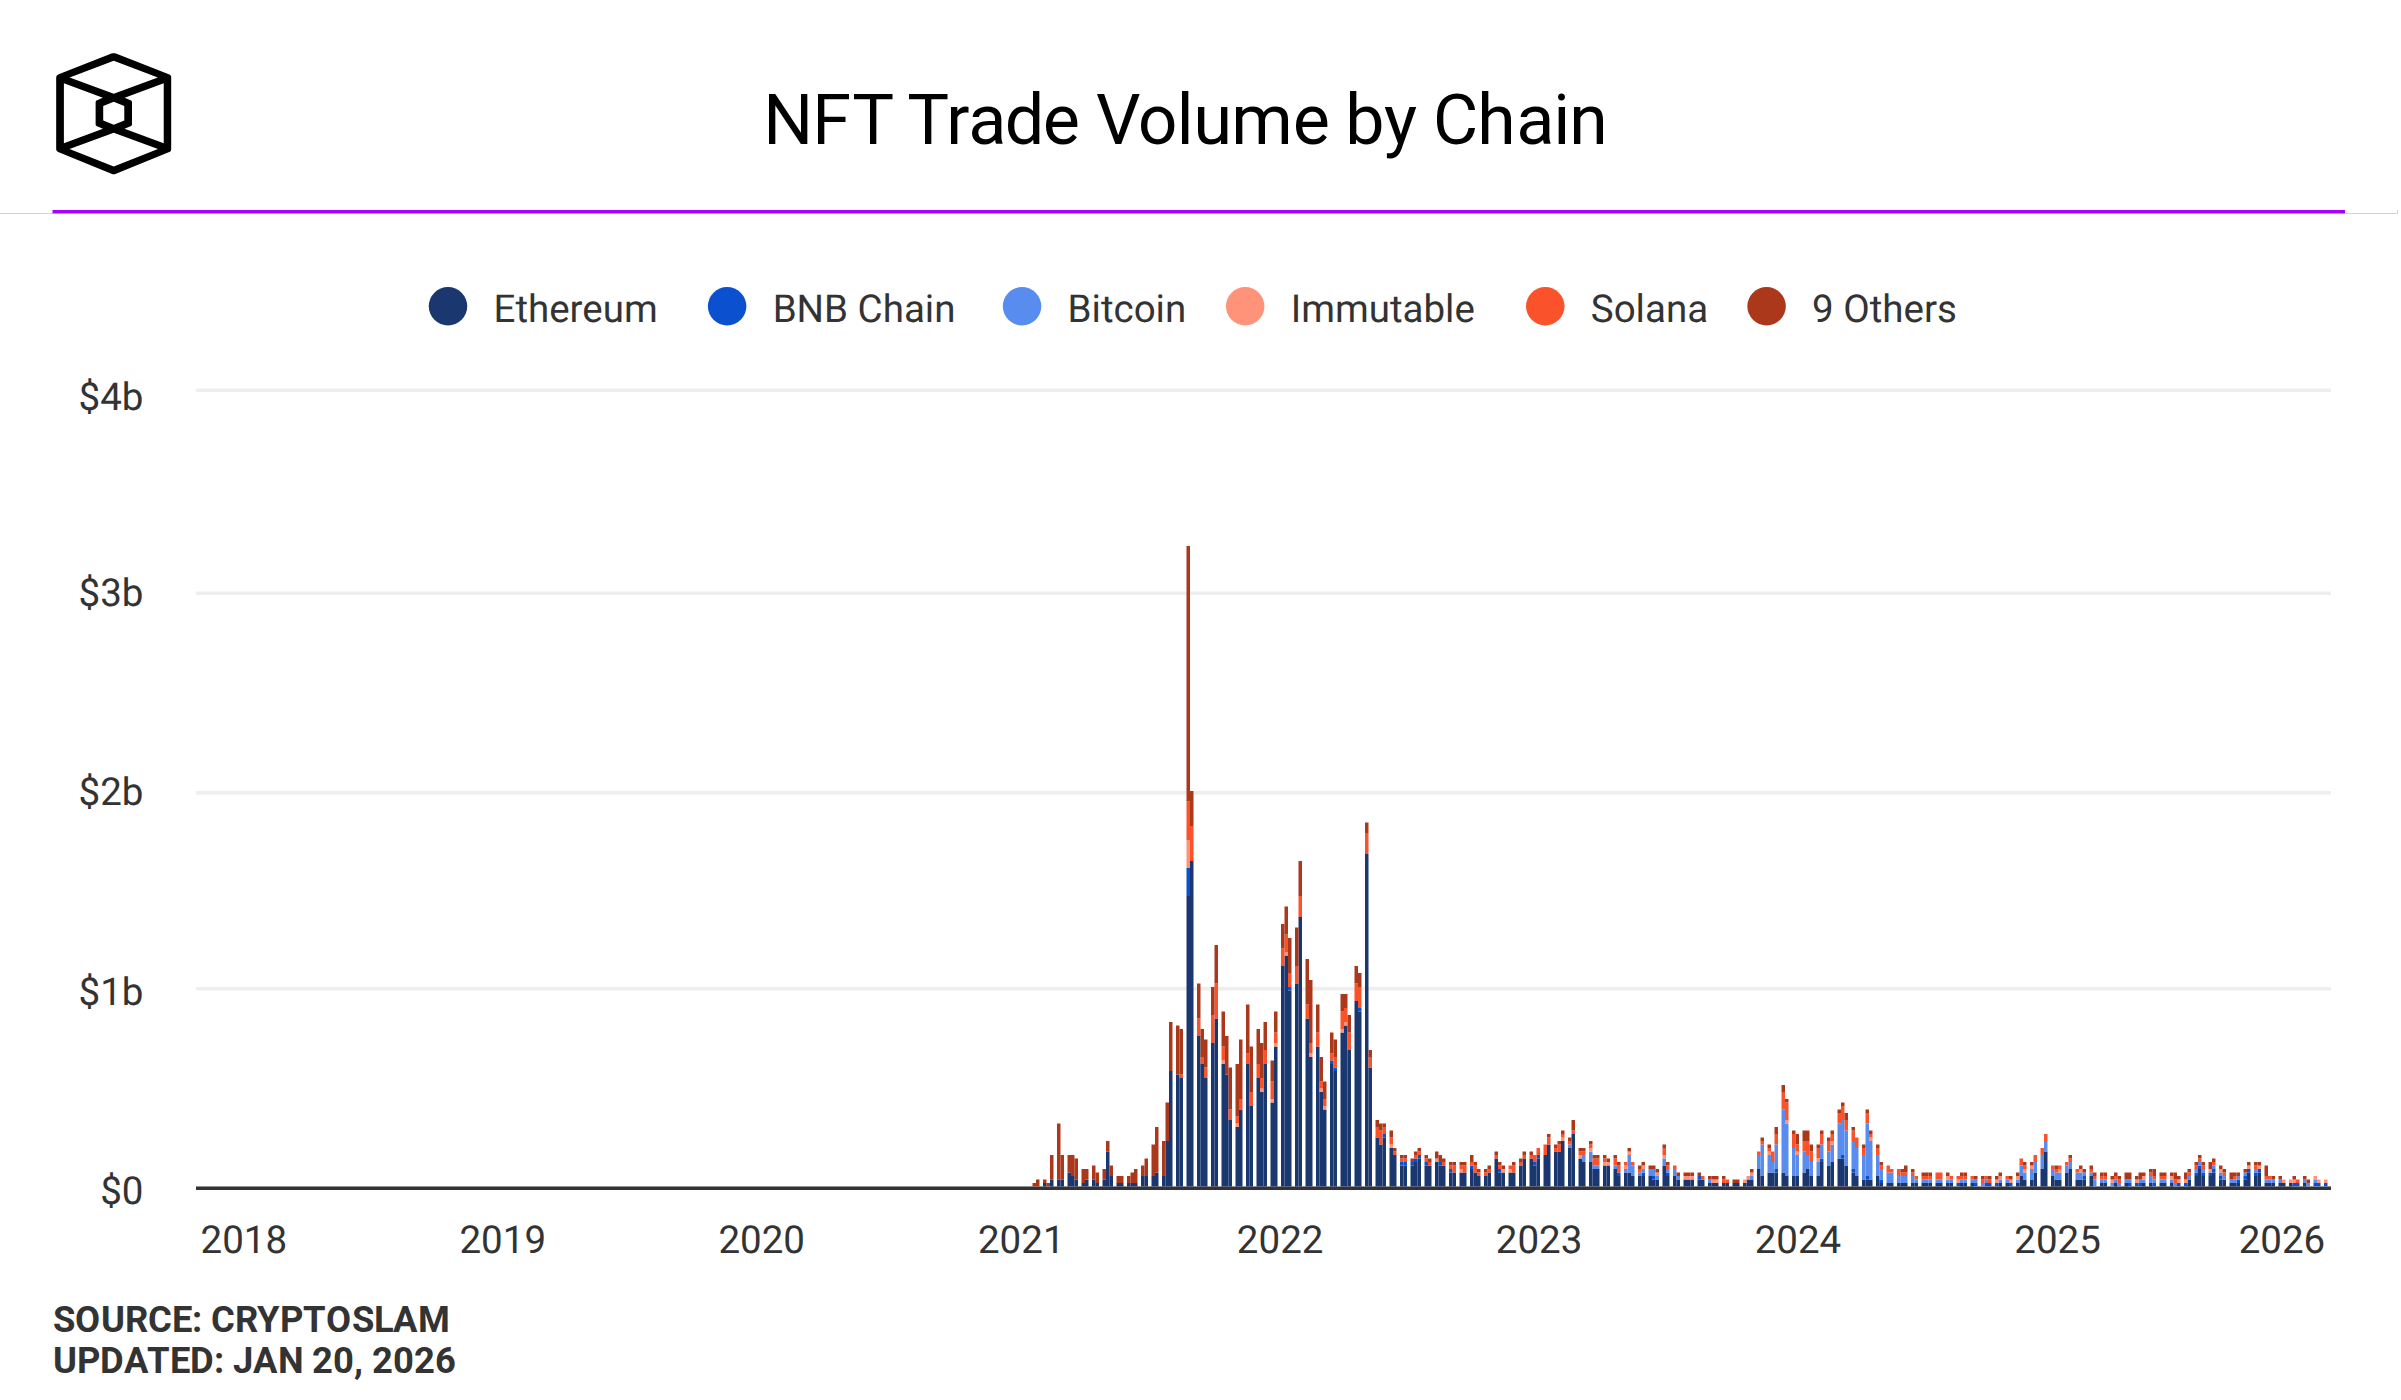
\includegraphics[width=.9\textwidth]{Figures/nft-trade-volume-by-chain.png}
  \end{figure}
  \textbf{What drove the boom}:
  \begin{itemize}
    \item Crypto bull market (wealth effect)
    \item Social signalling (profile-picture culture)
    \item Speculation and ``greater fool'' dynamics
    \item FOMO and media hype
  \end{itemize}
\end{frame}

\begin{frame}{The 2023 NFT Crash}
  \begin{figure}
    \centering
    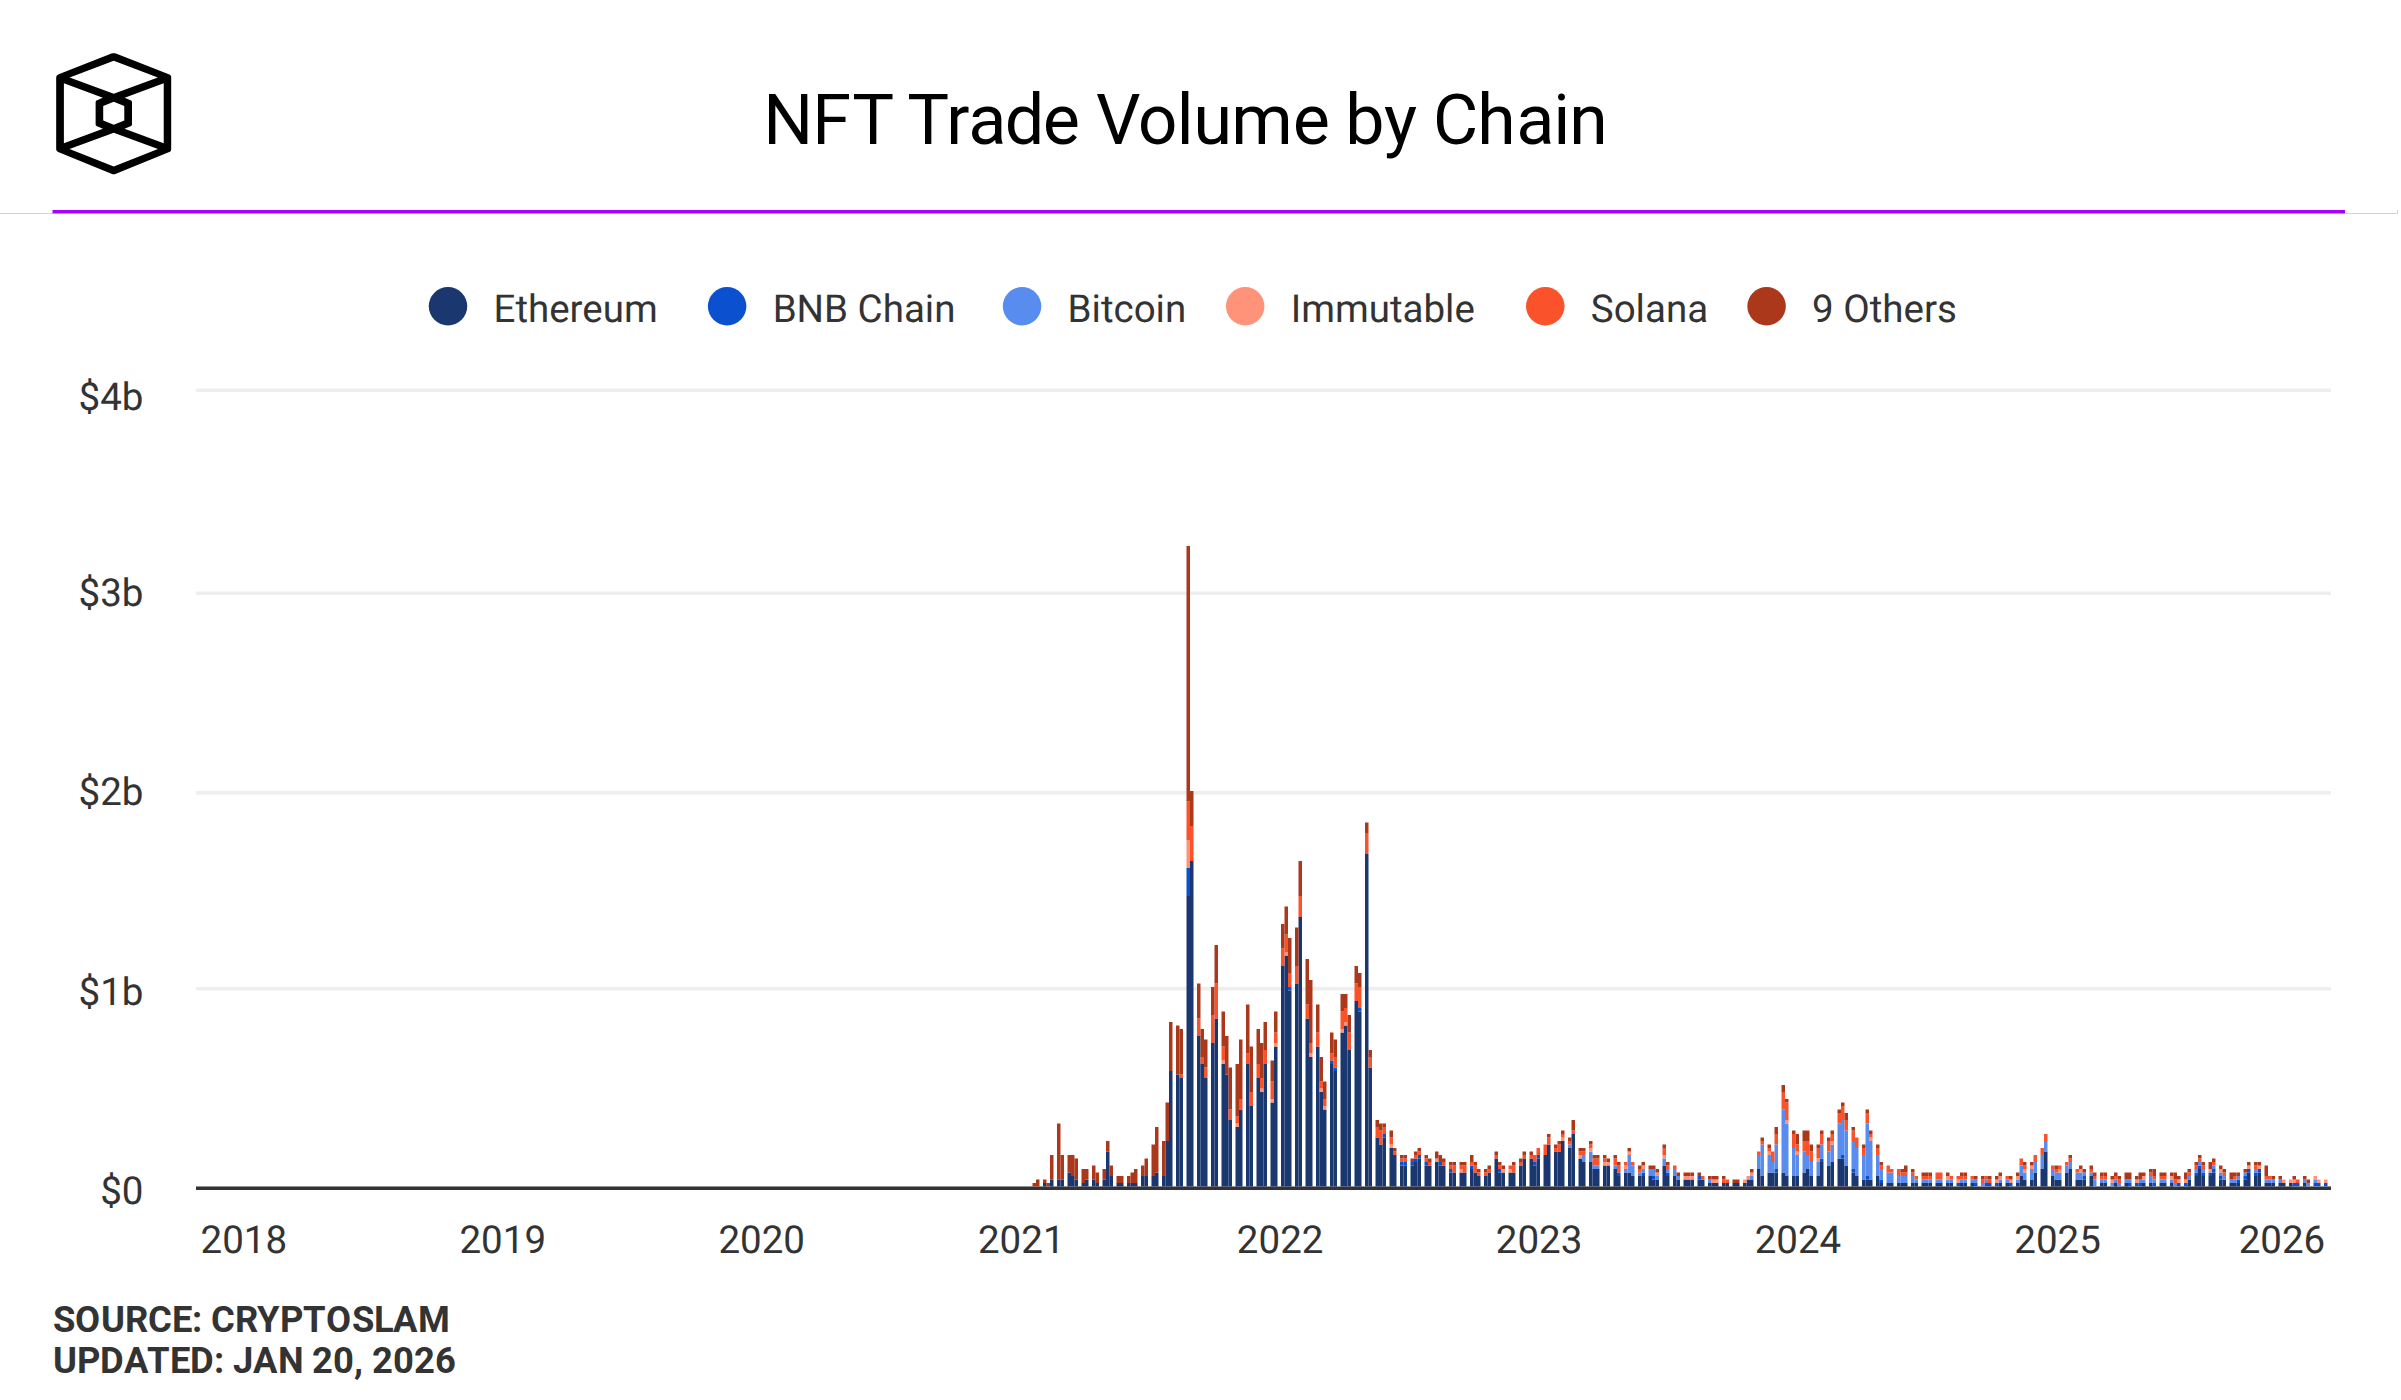
\includegraphics[width=.9\textwidth]{Figures/nft-trade-volume-by-chain.png}
  \end{figure}
  \textbf{What drove the crash}:
  \begin{itemize}
    \item Crypto winter reduced speculative capital
    \item Utility promises (games, metaverse) did not materialise
    \item Wash trading exposed---volumes were inflated
    \item Oversupply: too many collections, not enough buyers
  \end{itemize}
\end{frame}


\begin{frame}{The Wash Trading Problem}
  % [FIGURE 5: Estimated wash trading percentage in NFT markets]
  % Source: Chainalysis, Hildobby Dune dashboard
  
  \begin{block}{Wash Trading}
    Buying and selling an asset to yourself (or colluding parties) to create fake trading volume.
  \end{block}
  
  \vspace{0.5em}
  \textbf{Why it happened in NFTs}:
  \begin{itemize}
    \item Marketplace rewards (tokens, airdrops) based on volume
    \item Create appearance of liquidity and demand
    \item Manipulate ``floor price'' for collection
    \item Tax loss harvesting (in some jurisdictions)
  \end{itemize}
  
  \vspace{0.5em}
  \textbf{Scale}: studies estimate 40--80\% of NFT volume was wash trading at peak.
  
  \vspace{0.5em}
  \textbf{Detection}: Same wallet on both sides, circular transactions, economically irrational patterns, funded from same source.
\end{frame}

\begin{frame}{NFT Pricing: The Fundamental Challenge}
  \textbf{How do you value a unique asset with no cash flows?}
  
  \vspace{1em}
  Traditional valuation doesn't apply:
  \begin{itemize}
    \item No dividends $\rightarrow$ No DCF
    \item No earnings $\rightarrow$ No P/E ratio
    \item Unique items $\rightarrow$ No comparable sales (exactly)
  \end{itemize}
  
  \vspace{1em}
  \textbf{What drives NFT prices}:
  \begin{itemize}
    \item Rarity of traits (verifiable on-chain)
    \item Artist/creator reputation
    \item Collection brand and community
    \item Historical sales of similar items
    \item Social signaling value
    \item Speculation on future demand
  \end{itemize}
  
  \vspace{0.5em}
  \textbf{Result}: Prices are highly subjective and volatile---more art market than financial market.
\end{frame}

\begin{frame}{Lessons from the NFT Bubble}
  \textbf{What went wrong}:
  \begin{itemize}
    \item Speculation overwhelmed utility
    \item ``Community'' and ``roadmap'' promises were often empty
    \item Royalties weren't technically enforceable
    \item Legal status of ownership unclear
    \item Most buyers were speculators, not collectors
  \end{itemize}
  
  \vspace{1em}
  \textbf{What remains valuable}:
  \begin{itemize}
    \item The \textit{technology} of provable digital ownership
    \item Creator royalties \textit{concept} (even if enforcement failed)
    \item On-chain provenance and authenticity
    \item Programmable ownership rights
  \end{itemize}
  
  \vspace{0.5em}
  The infrastructure is useful. The 2021 use case (speculative JPEGs) was not sustainable.
\end{frame}

%----------------------------------------------------------------------------------------
\section{Real-World Asset (RWA) Tokenization}
%----------------------------------------------------------------------------------------

\begin{frame}{The Institutional Pivot}
  \begin{figure}
    \centering
    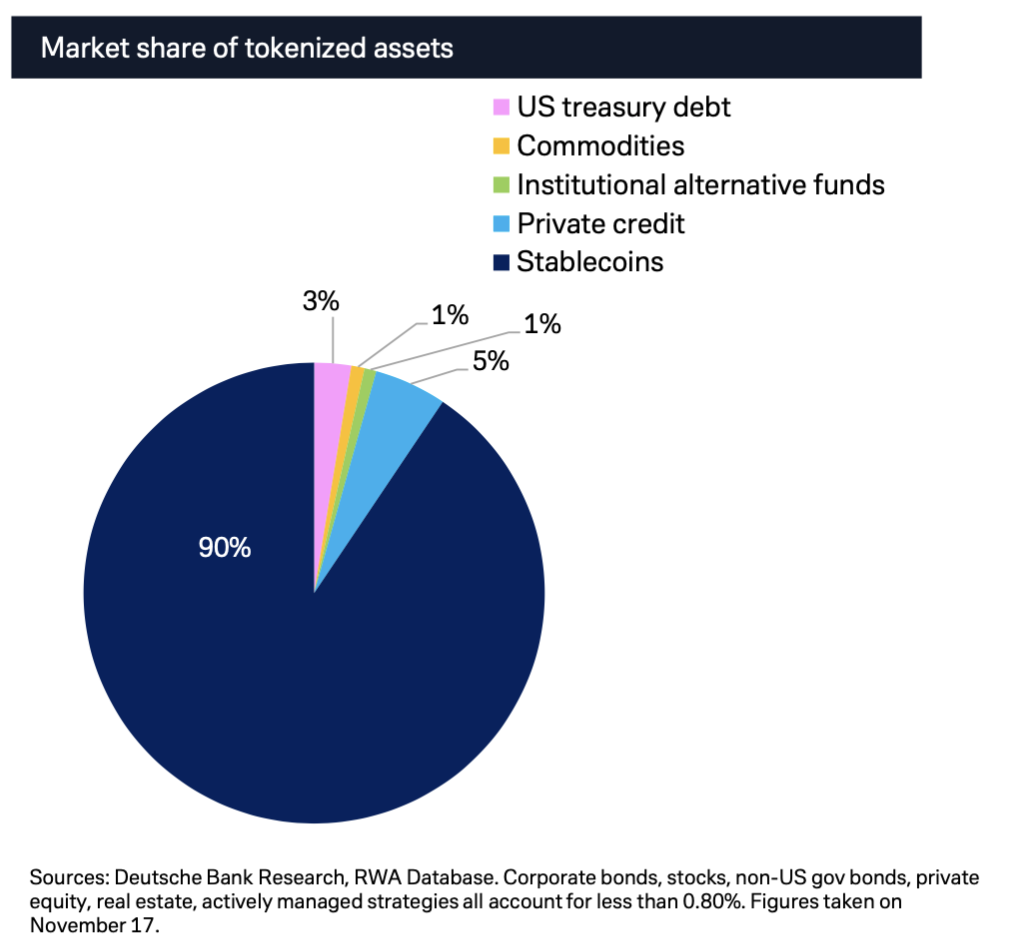
\includegraphics[width=.5\textwidth]{Figures/mkt share tokenization.png}
  \end{figure}

  \vspace{1em}
  \textbf{What is being tokenized}: US Treasury bills, corporate bonds, money market funds, real estate, private credit, and commodities.

  \vspace{1em}
  \textbf{Key players entering}: BlackRock (BUIDL fund), Franklin Templeton (on-chain money market fund), JPMorgan (Onyx platform), and Goldman Sachs (Digital Asset Platform).
\end{frame}



\begin{frame}{Tokenized Treasuries: The Killer Use Case?}
  % [FIGURE 7: Tokenized treasury market growth chart]
  % Source: rwa.xyz, Steakhouse Financial
  
  \textbf{What it is}: US Treasury bills represented as tokens on a blockchain.
  
  \vspace{0.5em}
  \textbf{How it works}:
  \begin{enumerate}
    \item Issuer (e.g., BlackRock) buys T-bills
    \item Issues tokens representing shares in the T-bill portfolio
    \item Token holders receive yield (distributed on-chain)
    \item Tokens can be transferred 24/7
  \end{enumerate}
  
  \vspace{0.5em}
  \textbf{Why it matters}:
  \begin{itemize}
    \item DeFi protocols can hold yield-bearing collateral
    \item 24/7 settlement (vs T+1 for traditional)
    \item Programmable: Auto-reinvest, use as collateral
    \item Global access to US government debt
  \end{itemize}
  
  \vspace{0.5em}
  \textbf{Market size} (2024): $\approx$\$1.5 billion in tokenized treasuries.
\end{frame}

\begin{frame}{Case Study: BlackRock BUIDL}
  \textbf{BUIDL} (BlackRock USD Institutional Digital Liquidity Fund)
  
  \vspace{0.5em}
  Launched March 2024 on Ethereum.
  
  \vspace{1em}
  \textbf{Structure}:
  \begin{itemize}
    \item Invests in T-bills, repos, cash
    \item Each BUIDL token = \$1 (stable NAV)
    \item Daily accrued dividends (paid monthly)
    \item Tokenised by Securitize
  \end{itemize}
  
  \vspace{0.5em}
  \textbf{Requirements}:
  \begin{itemize}
    \item Qualified purchasers only (\$5M+ investable assets)
    \item \$5 million minimum investment
    \item KYC/AML through Securitize
  \end{itemize}
  
  \vspace{0.5em}
  \textbf{Significance}: World's largest asset manager tokenizing products on public blockchain. Signal of institutional legitimacy.
\end{frame}

\begin{frame}{Why Tokenize Real-World Assets?}
  % [FIGURE 8: Comparison diagram - traditional vs tokenized settlement]
  % Can create in TikZ
  
  \begin{center}
  \begin{tabular}{lcc}
    \toprule
    & \textbf{Traditional} & \textbf{Tokenized} \\
    \midrule
    Settlement & T+1 or T+2 & Near-instant \\
    Trading hours & Market hours & 24/7/365 \\
    Minimum investment & Often \$1,000+ & Can be \$1 \\
    Fractional ownership & Limited & Native \\
    Cross-border & Complex, expensive & Simplified \\
    Transparency & Periodic reports & Real-time on-chain \\
    Programmability & None & Smart contracts \\
    \bottomrule
  \end{tabular}
  \end{center}
  
  \vspace{0.5em}
  \textbf{The promise}: More efficient capital markets with lower friction, broader access, and automated compliance.
\end{frame}

\begin{frame}{RWA Tokenization Challenges}
  \textbf{Legal and regulatory}:
  \begin{itemize}
    \item What does the token legally represent?
    \item Securities law compliance
    \item Cross-jurisdictional recognition
    \item Bankruptcy treatment
  \end{itemize}
  
  \vspace{0.5em}
  \textbf{Technical}:
  \begin{itemize}
    \item Oracle problem: Who verifies the off-chain asset exists?
    \item Custody of underlying assets
    \item Blockchain scalability and costs
    \item Interoperability between chains
  \end{itemize}
  
  \vspace{0.5em}
  \textbf{Market structure}:
  \begin{itemize}
    \item Liquidity fragmentation
    \item Need for qualified custodians
    \item Integration with existing financial infrastructure
  \end{itemize}
  
  \vspace{0.5em}
  Tokenization doesn't eliminate counterparty risk---it just moves it.
\end{frame}

%----------------------------------------------------------------------------------------
\section{Security Tokens}
%----------------------------------------------------------------------------------------

\begin{frame}{What Are Security Tokens?}
  \begin{block}{Security Token}
    A token that represents ownership in a regulated security---equity, debt, or investment contract---and is subject to securities law.
  \end{block}
  
  \vspace{1em}
  \textbf{Key distinction}:
  \begin{itemize}
    \item \textbf{Utility token}: Access to a product/service (maybe not a security)
    \item \textbf{Security token}: Investment contract, ownership stake (definitely a security)
  \end{itemize}
  
  \vspace{1em}
  \textbf{The Howey Test} (US): Is it an ``investment of money in a common enterprise with expectation of profits from efforts of others''?
  
  \vspace{0.5em}
  If yes $\rightarrow$ It's a security $\rightarrow$ Must comply with securities law.
\end{frame}

\begin{frame}{Initial Coin Offerings (ICOs)}
  \begin{block}{Initial Coin Offering (ICO)}
    A fundraising method where a project sells newly created tokens to investors in exchange for cryptocurrency (usually ETH or BTC), typically before the product is built.
  \end{block}
  
  \vspace{0.5em}
  \textbf{How it worked} (2017 boom):
  \begin{enumerate}
    \item Project publishes a ``whitepaper'' describing the idea
    \item Investors send ETH to a smart contract
    \item Investors receive new tokens in return
    \item Tokens trade on exchanges (often immediately)
  \end{enumerate}

  \vspace{0.5em}
  \textbf{The 2017 ICO boom}:
  \begin{itemize}
    \item Over \$6 billion raised in 2017 alone
    \item Many projects had no working product
    \item Anyone could participate---no investor protections
    \item Examples: EOS (\$4B), Tezos (\$232M), Filecoin (\$257M)
  \end{itemize}
  
  \vspace{0.5em}
  \textbf{The problem}: Most ICO tokens were likely \highlight{unregistered securities}.
\end{frame}

\begin{frame}{The ICO Regulatory Crackdown}
  % [FIGURE: SEC enforcement actions or ICO market collapse chart]
  % Source: ICObench, SEC press releases
  
  \textbf{SEC position} (2017-2018): Most ICO tokens are securities.
  
  \vspace{0.5em}
  \textbf{The DAO Report} (July 2017): SEC ruled that DAO tokens were securities, signaling that securities laws apply to token sales.
  
  \vspace{0.5em}
  \textbf{Enforcement actions}:
  \begin{itemize}
    \item Munchee (2017): Shut down, returned \$15M to investors
    \item Paragon, Airfox (2018): \$250K penalties each
    \item Block.one/EOS (2019): \$24M settlement
    \item Telegram/TON (2020): \$1.2B returned, project cancelled
    \item Ripple/XRP (2020): Ongoing lawsuit
  \end{itemize}
  
  \vspace{0.5em}
  \textbf{Result}: ICO market collapsed. Projects seeking compliant fundraising turned to \textbf{Security Token Offerings (STOs)}.
\end{frame}

\begin{frame}{Security Token Offerings (STOs) vs ICOs}
  % [FIGURE 9: Timeline showing ICO boom (2017) → regulatory crackdown → STO emergence]
  % Can create in TikZ
  
  \begin{center}
  \resizebox{1\textwidth}{!}{\begin{tabular}{lll}
    \toprule
    & \textbf{ICO (2017)} & \textbf{STO} \\
    \midrule
    Regulatory status & Often unclear/non-compliant & Registered or exempt \\
    Investor requirements & Anyone & Often accredited only \\
    Disclosure & Whitepaper (variable quality) & Prospectus/offering memo \\
    Investor protection & Minimal & Securities law applies \\
    Secondary trading & Unregulated exchanges & Licensed platforms \\
    \bottomrule
  \end{tabular}}
  \end{center}
  
  \vspace{0.5em}
  \textbf{US exemptions used for STOs}:
  \begin{itemize}
    \item Reg D (accredited investors only)
    \item Reg A+ (mini-IPO, up to \$75M)
    \item Reg S (non-US investors)
  \end{itemize}
\end{frame}

\begin{frame}{Security Token Infrastructure}
  \textbf{Issuance platforms}: Securitize, Polymath, Harbor
  
  \vspace{0.5em}
  \textbf{Key requirements}:
  \begin{itemize}
    \item KYC/AML verification of all token holders
    \item Transfer restrictions (only to verified wallets)
    \item Compliance with holding periods (e.g., Reg D lockup)
    \item Cap table management
    \item Reporting and disclosure
  \end{itemize}
  
  \vspace{1em}
  \textbf{How it works technically}:
  \begin{itemize}
    \item Whitelist of approved addresses
    \item Transfer function checks compliance before executing
    \item Forced transfers possible (for legal requirements)
    \item Dividend/interest distribution automated
  \end{itemize}
  
  \vspace{0.5em}
  This is \textit{permissioned} tokenization---not the ``anyone can participate'' ethos of DeFi.
\end{frame}

\begin{frame}{Security Tokens: Current State}
  \textbf{What's been tokenized}:
  \begin{itemize}
    \item Real estate (commercial and residential)
    \item Private company equity
    \item Fund shares
    \item Corporate bonds
    \item Revenue-sharing agreements
  \end{itemize}
  
  \vspace{0.5em}
  \textbf{Challenges}:
  \begin{itemize}
    \item Limited secondary market liquidity
    \item High compliance costs relative to deal size
    \item Fragmented regulatory landscape globally
    \item Chicken-and-egg: Need liquidity to attract issuers, need issuers to build liquidity
  \end{itemize}
  
  \vspace{1em}
  \textbf{Outlook}: Security tokens are growing but remain niche. Institutional adoption (BlackRock, etc.) may be the catalyst for broader growth.
\end{frame}

%----------------------------------------------------------------------------------------
\section{Practical Applications}
%----------------------------------------------------------------------------------------

\begin{frame}{Digital Art and Collectibles}
  % [FIGURE 10: Examples of notable NFT art sales with caveats]
  
  \textbf{The original NFT use case}---still relevant, but with caveats.

  \begin{figure}
    \centering
    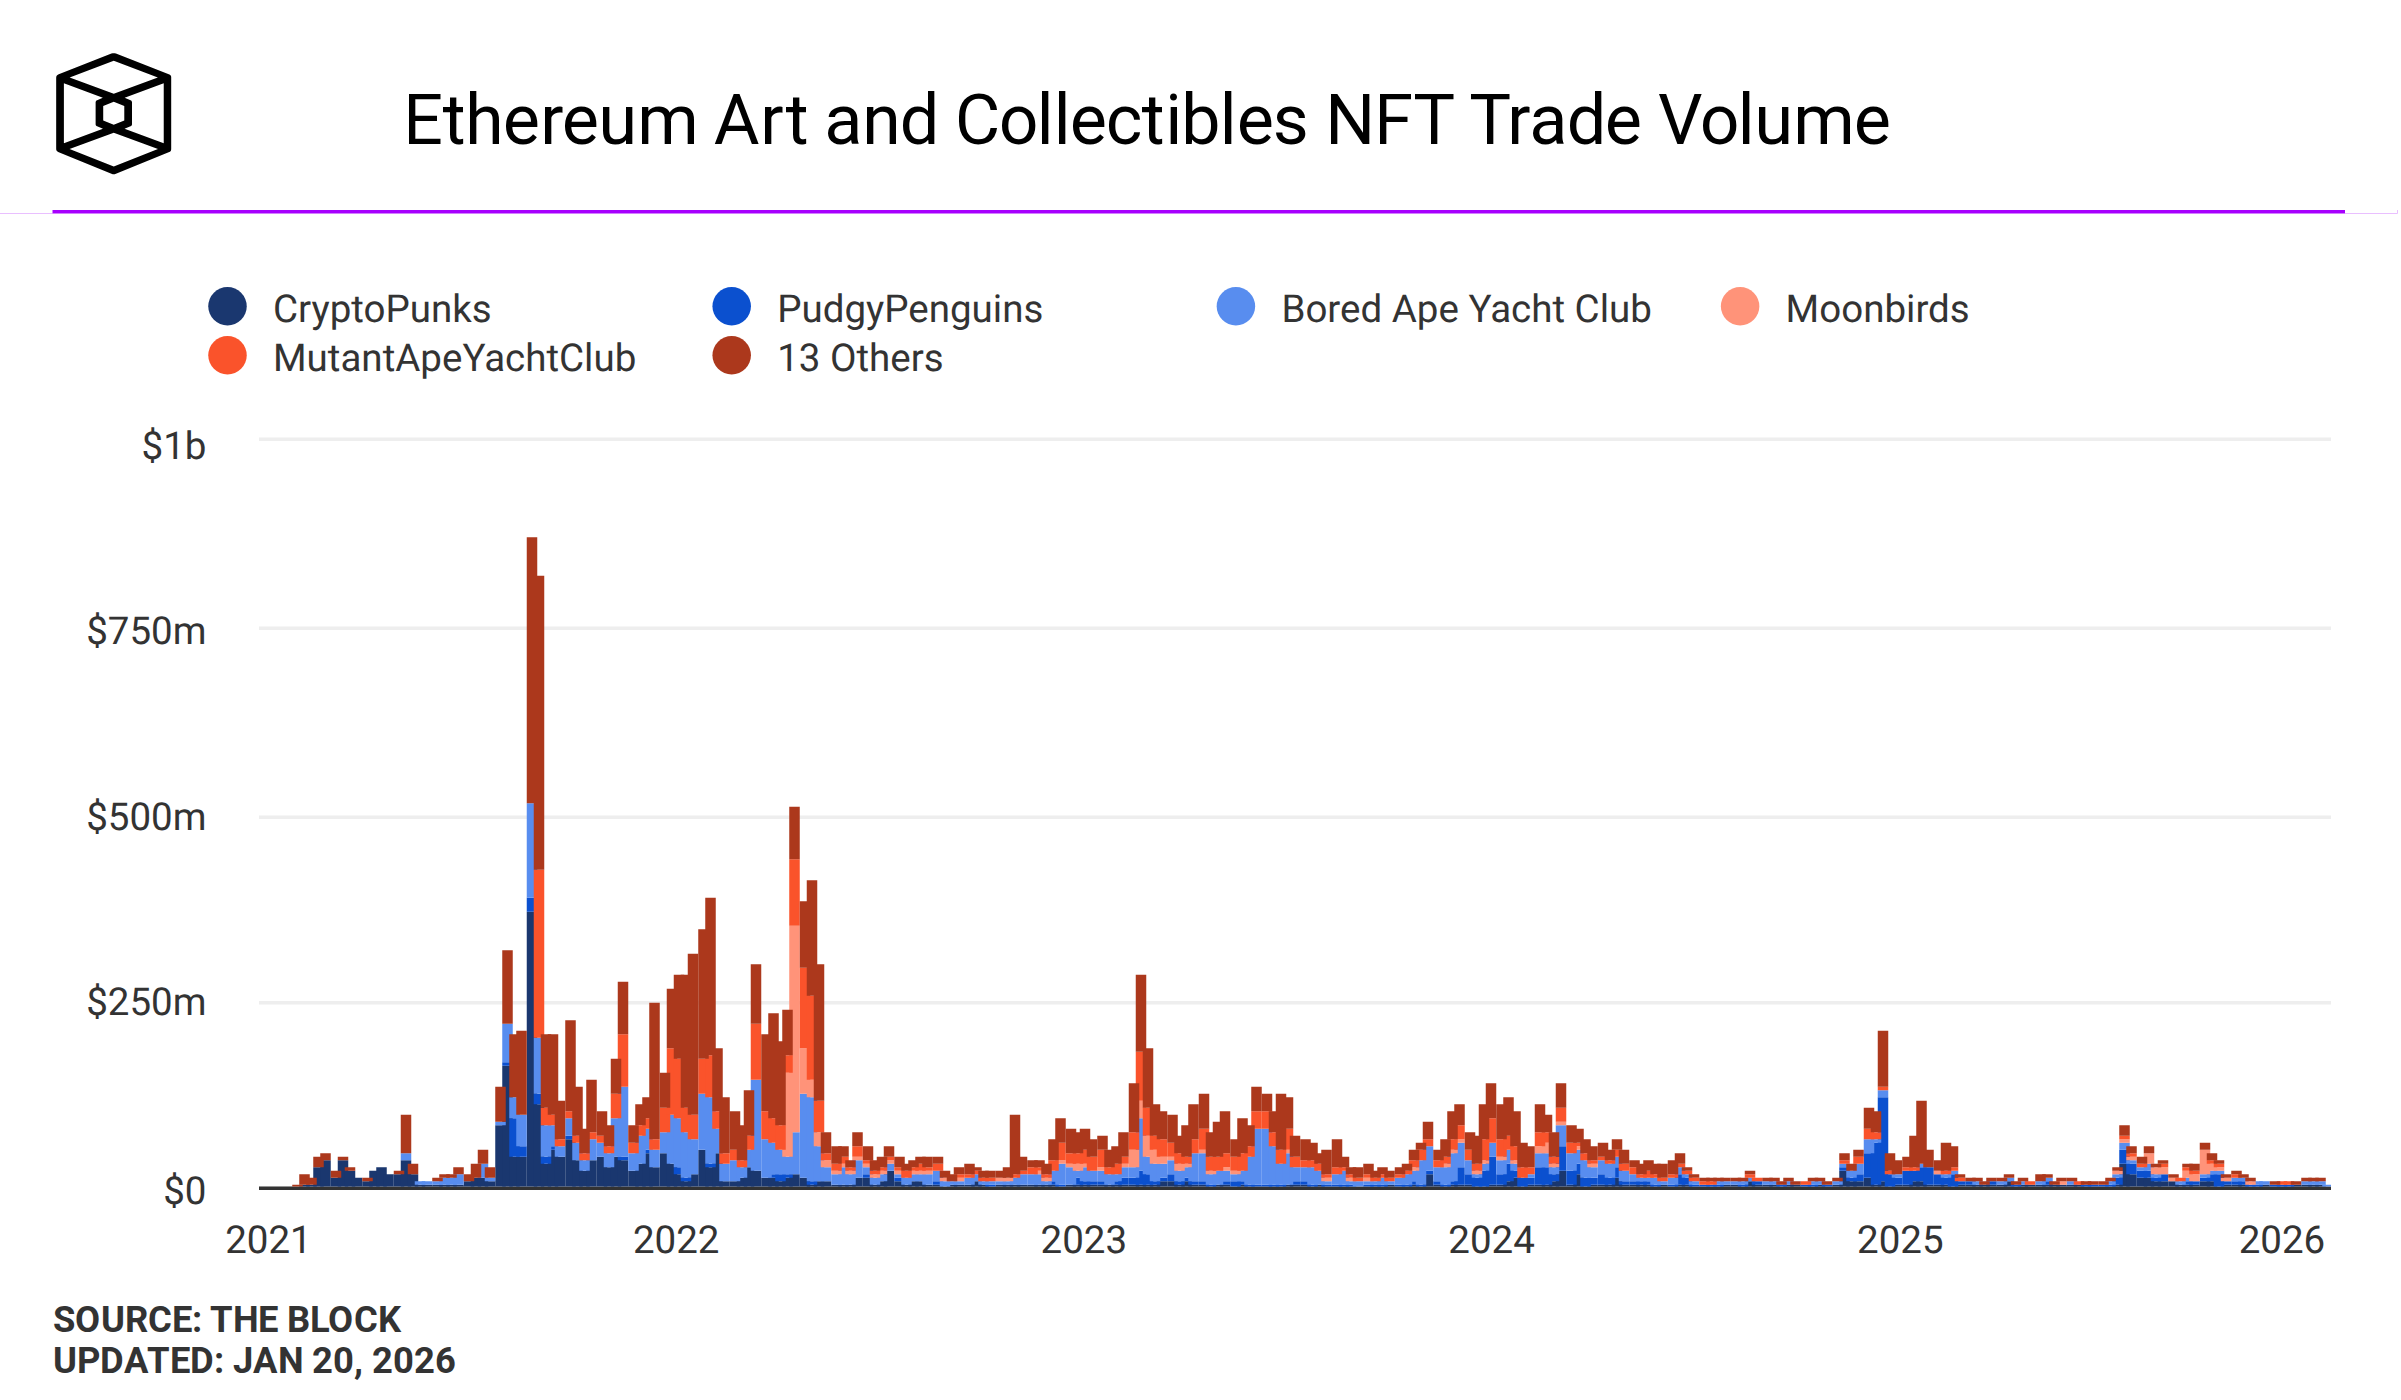
\includegraphics[width=.75\textwidth]{Figures/ethereum-art-and-collectibles-nft-trade-volume.png}
  \end{figure}

  \begin{itemize}
    \item\textbf{What works}: Provenance tracking for digital art, direct artist-to-collector sales, global market access
    \item\textbf{What doesn't}: Speculation-driven pricing, copyright isn't transferred (usually), right-click-save ``problem'' (social, not technical)
%    \item \textbf{Sustainable use}: Art market (galleries, auctions) adopting NFTs for authentication and provenance, not speculation.
  \end{itemize}
  
\end{frame}

\begin{frame}{Supply Chain and Provenance}
  \textbf{Use case}: Track products from origin to consumer.
  
  \vspace{0.5em}
  \textbf{Examples}:
  \begin{itemize}
    \item Luxury goods authentication (LVMH's Aura)
    \item Food traceability (Walmart + IBM Food Trust)
    \item Pharmaceutical supply chain
    \item Conflict mineral tracking
  \end{itemize}
  
  \vspace{0.5em}
  \textbf{How it works}:
  \begin{itemize}
    \item Each product gets a unique token/identifier
    \item Each handoff recorded on-chain
    \item Consumer can verify full history
  \end{itemize}
  
  \vspace{0.5em}
  \textbf{Limitation}: The oracle problem again. Blockchain can't verify that the physical item matches the digital record. Still requires trusted inputs.
  
  \vspace{0.5em}
  ``Garbage in, garbage out''---immutably recorded on a blockchain.
\end{frame}

\begin{frame}{Fractional Ownership}
  \textbf{Idea}: Tokenize expensive assets, sell fractions.
  
  \vspace{0.5em}
  \textbf{Examples}:
  \begin{itemize}
    \item Real estate: Own 0.1\% of a building
    \item Art: Own shares in a Picasso
    \item Collectibles: Fractional sports memorabilia
  \end{itemize}
  
  \vspace{0.5em}
  \textbf{Benefits}:
  \begin{itemize}
    \item Lower minimum investment
    \item Diversification possible
    \item Liquidity for illiquid assets
  \end{itemize}
  
  \vspace{0.5em}
  \textbf{Challenges}:
  \begin{itemize}
    \item Securities law applies (usually)
    \item Governance: Who decides to sell the underlying?
    \item Custody and insurance of physical asset
    \item Thin secondary markets
  \end{itemize}
  
  \vspace{0.5em}
  \textbf{Reality}: Fractionalization has existed pre-blockchain (REITs, art funds). Tokenization adds programmability and potentially broader access.
\end{frame}

%----------------------------------------------------------------------------------------
\section{Challenges and Future}
%----------------------------------------------------------------------------------------

\begin{frame}{The Oracle Problem (Again)}
\begin{center}
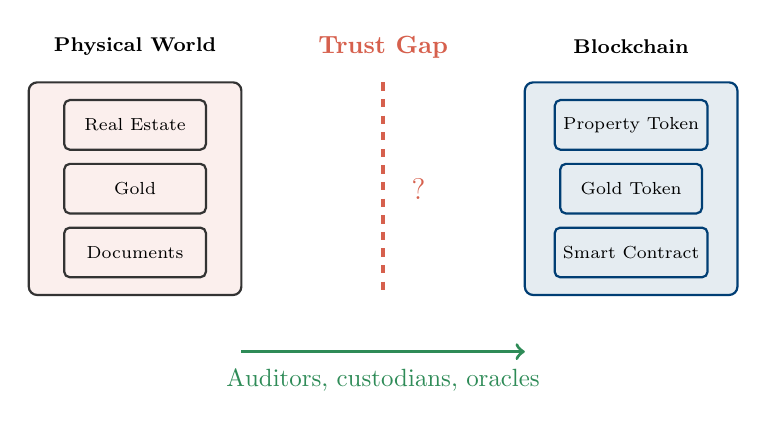
\begin{tikzpicture}[scale=0.9, transform shape,
    physbox/.style={rectangle, draw=DarkGray, fill=AccentOrange!10, thick, minimum width=2cm, minimum height=0.7cm, align=center, font=\scriptsize, rounded corners=2pt},
    chainbox/.style={rectangle, draw=ImperialBlue, fill=ImperialBlue!10, thick, minimum width=2cm, minimum height=0.7cm, align=center, font=\scriptsize, rounded corners=2pt}
]

% Physical World
\node[font=\footnotesize\bfseries] at (-3.5, 2.5) {Physical World};
\draw[thick, DarkGray, fill=AccentOrange!10, rounded corners=3pt] (-5, -1) rectangle (-2, 2);
\node[physbox] at (-3.5, 1.4) {Real Estate};
\node[physbox] at (-3.5, 0.5) {Gold};
\node[physbox] at (-3.5, -0.4) {Documents};

% Blockchain
\node[font=\footnotesize\bfseries] at (3.5, 2.5) {Blockchain};
\draw[thick, ImperialBlue, fill=ImperialBlue!10, rounded corners=3pt] (2, -1) rectangle (5, 2);
\node[chainbox] at (3.5, 1.4) {Property Token};
\node[chainbox] at (3.5, 0.5) {Gold Token};
\node[chainbox] at (3.5, -0.4) {Smart Contract};

% Gap
\draw[very thick, AccentOrange, dashed] (0, 2) -- (0, -1);
\node[font=\bfseries, AccentOrange] at (0, 2.5) {Trust Gap};
\node[font=\large, AccentOrange] at (0.5, 0.5) {?};

% Bridge
\draw[very thick, AccentGreen, ->] (-2, -1.8) -- (2, -1.8);
\node[AccentGreen] at (0, -2.2) {Auditors, custodians, oracles};

\end{tikzpicture}
\end{center}

\vspace{0.3em}
\textbf{Fundamental challenge}: Blockchains can only verify on-chain data.

\vspace{0.3em}
For tokenized real-world assets, someone must verify: Does the asset exist? Is it authentic? Who owns it legally?

\vspace{0.3em}
\highlight{Tokenization doesn't eliminate trust---it shifts it.}
\end{frame}




\begin{frame}{Legal Status of Tokenized Ownership}
  \textbf{Key questions} (often unresolved):
  \begin{itemize}
    \item Does the token holder have legal title to the underlying?
    \item What happens in bankruptcy?
    \item Which jurisdiction's law applies?
    \item How are disputes resolved?
    \item Is the token itself property?
  \end{itemize}
  
  \vspace{0.5em}
  \textbf{Current approaches}:
  \begin{itemize}
    \item Token represents contractual claim (not direct ownership)
    \item SPV structure: Token = shares in entity that owns asset
    \item Legal wrapper with token as ``digital twin''
  \end{itemize}
  
  \vspace{0.5em}
  \textbf{Regulatory developments}:
  \begin{itemize}
    \item MiCA (EU): Framework for crypto-assets
    \item UK Law Commission: Recognising digital assets as property
    \item Wyoming: DAO and digital asset laws
  \end{itemize}
\end{frame}

\begin{frame}{Interoperability and Fragmentation}
  \textbf{Problem}: Assets tokenized on different chains can't easily interact.
  
  \vspace{0.5em}
  \textbf{Current state}:
  \begin{itemize}
    \item Ethereum dominates but has high fees
    \item L2s (Arbitrum, Optimism, Base) growing
    \item Alternative L1s (Solana, Avalanche) have separate ecosystems
    \item Private/permissioned chains for institutions
  \end{itemize}
  
  \vspace{0.5em}
  \textbf{Bridging solutions}:
  \begin{itemize}
    \item Cross-chain bridges (but security risks)
    \item Multi-chain token deployments
    \item Interoperability protocols (Chainlink CCIP, LayerZero)
  \end{itemize}
  
  \vspace{0.5em}
  \textbf{For RWA tokenization}: Institutions may prefer private chains for control, but this limits composability with DeFi.
\end{frame}

\begin{frame}{The Future of Tokenization}
  \textbf{Near-term} (2-5 years):
  \begin{itemize}
    \item Tokenized treasuries and money market funds scale
    \item More traditional asset managers enter
    \item Regulatory clarity improves (MiCA implementation)
    \item Security token infrastructure matures
  \end{itemize}
  
  \vspace{0.5em}
  \textbf{Medium-term} (5-10 years):
  \begin{itemize}
    \item Broader asset classes tokenized (private equity, real estate)
    \item Integration with traditional financial infrastructure
    \item CBDCs potentially interoperating with tokenized assets
    \item Credentials and identity (SBTs) gain adoption
  \end{itemize}
  
  \vspace{0.5em}
  \textbf{Key question}: Will tokenization happen on public blockchains (Ethereum) or private/permissioned systems? The answer affects decentralisation, access, and composability.
\end{frame}

%----------------------------------------------------------------------------------------
\section{Summary}
%----------------------------------------------------------------------------------------

\begin{frame}{Key Takeaways}
  \begin{enumerate}
    \item \textbf{Tokenization = digital ownership on blockchain}
    \begin{itemize}
      \item Fungible (ERC-20) vs non-fungible (ERC-721) vs multi-token (ERC-1155)
    \end{itemize}
    
    \vspace{0.3em}
    \item \textbf{NFT speculation crashed, but technology remains}
    \begin{itemize}
      \item Wash trading, hype, and unsustainable economics
      \item Provable digital ownership is still valuable
    \end{itemize}
    
    \vspace{0.3em}
    \item \textbf{Real-world asset tokenization is growing}
    \begin{itemize}
      \item Tokenized treasuries: BlackRock, Franklin Templeton
      \item Security tokens: Regulated, compliant, but limited liquidity
    \end{itemize}
    
    \vspace{0.3em}
    \item \textbf{Practical applications beyond speculation}
    \begin{itemize}
      \item Credentials (SBTs), supply chain, fractional ownership
    \end{itemize}
    
    \vspace{0.3em}
    \item \textbf{Challenges remain}: Oracle problem, legal status, interoperability
  \end{enumerate}
\end{frame}

\begin{frame}{What's Next}
  \textbf{Topic 7: Cryptocurrency Investment}
  \begin{itemize}
    \item Market structure and trading venues
    \item Valuation approaches (or lack thereof)
    \item Risk factors and portfolio considerations
    \item ETFs and institutional products
  \end{itemize}
  
  \vspace{1em}
  \textbf{Preparation}:
  \begin{itemize}
    \item Think about: How would you value Bitcoin? Is it like gold, a currency, a tech stock, or something else entirely?
    \item Explore: Look at Bitcoin and Ethereum ETF flows since approval
  \end{itemize}
\end{frame}

\begin{frame}[plain]
  \vfill
  \begin{center}
    {\Large Questions?}
  \end{center}
  \vfill
\end{frame}

\end{document}